
\documentclass[utf8]{beamer}

\usepackage{beamerthemesplit}
\usepackage[absolute]{textpos}

\title{Collocation Extraction: A study for the Unitex project}
\author{B.Burak Arslan}
\institute{Marne-la-Vall\'{e}e University, Paris}
\date{\today}
\bibliographystyle{abbrv}

\setbeamercovered{ transparent=20 }

\begin{document}
\frame{
	\titlepage
}

\frame{
	\frametitle{Outline}
	\tableofcontents
}
\section{Collocations}
\subsection{Definitions}
\frame{
	\frametitle{ Collocations: An Intuitive Definition }
	\begin{itemize}
	\item The term collocation (aka compound word or multi-word expression) is used to represent groups of words that either have slightly different meanings when used together, or have become idiosyncratic with heavy use.
	\item Has been an active research area even before the computing era.
	\item Noticed first as language constructs that, when translated word-by-word from a source language, stand out as awkward at best, for a native speaker of the target language.
	\end{itemize}
}
\frame{
	\frametitle{ Collocations: More Formal Definitions }
	\begin{itemize}
	\item ``Recurrent combinations of words that co-occur more often than expected by chance and that correspond to arbitrary word usages''	\cite{smadja93}
		\begin{itemize}
			\item later research has shown that collocations that do not manifest any statistical property also seem to exist \cite{1118854}.
		\end{itemize}
	\item ``Idiosyncratic interpretations that cross word boundaries''\cite{sag02multiword} 
		\begin{itemize}
			\item More accurate, but more vague and harder to track computationally
		\end{itemize}
	\end{itemize}
}
\subsection{Properties}
\frame{
	\frametitle{ Collocations: Properties }
	\begin{itemize}
	\item Study of the collocations in the pre-computing era showed that collocations have particular statistical distributions\cite{smadja93}.
		\begin{itemize}
			\item However, later research showed that collocations may not always carry statistical properties, or may be extremely sparse, even in fairly large corpora\cite{1118854}.
		\end{itemize}

	\item There is no general form that defines all collocations. They vary between two extremes, based on their rigidness in form\cite{sag02multiword}.
		\begin{itemize}
			\item Between Words-with-spaces and syntactically-flexible expressions
		\end{itemize}

	\item Collocations can only be learned by observing their occurrence in language use; they are otherwise not predictable\cite{seretan2003}.

	\end{itemize}
}

\section{Collocation Extraction Systems}
\subsection{Overview}
\frame{
	\frametitle{ Overview I }
	\begin{itemize}
	\item Requires both statistical and linguistic information in order to be successful.
	\item Basically, all of the collocation extraction systems that I reviewed work in three steps:
		\begin{enumerate}
		\item Identifying two-word collocation candidates
		\item Eliminating them
		\item Combining them to collocations that may span more words than two.
		\end{enumerate}
	\end{itemize}
} 
\frame{
	\frametitle{ Overview II }
	\begin{itemize}
		\item The defining steps being identification and elimination, the two may be undistinguishable. Two main approaches exist:
			\begin{itemize}
			\item Deep parsing
			\item Shallow Parsing 
			\end{itemize}
		\item I have tried to take the path of shallow parsing, but tried not to introduce any artifical constraints for simplifying memory management.
	\end{itemize}
} 
\subsection{Implementation}
\frame{
	\frametitle{ Preprocessing }
	\begin{itemize}
		\item As a first step the following preprocessing operations are applied:
			\begin{itemize}
			\item Normalization
			\item Tokenization
			\item Detection of Sentence Boundaries
			\item Lemmatization/POS Tagging
				\begin{itemize}
				\item  Introduces ambiguities that are stored in sentence automata.
				\end{itemize}
			\end{itemize}

	\end{itemize}
}

\frame{
	\frametitle{ Collocation Extraction }
	\begin{itemize}
		\item \texttt{Colloc} creates commutative pairs, than counts their number of occurences, never combining two different interpretations of the same word. 
		\item Every \textbf{unique} word combination consumes memory.
		\item This is where the memory needs may be more than typical.
		\item So a precaution that I call \textbf{compacting} is taken.
	\end{itemize}
}
\frame{
	\frametitle{ Compacting }
	\begin{itemize}
		\item Assuming that a $N$ phrase subset of the corpus exhibits the same statistical properties as the whole corpus itself, \texttt{Colloc} may delete, every $N$ sententences, combinations that have frequency values below $$(i-s)\frac{t}{e}$$

		where	
		\begin{description}
			\item[$i$] is the current number of the sentence
			\item[$s$] is the number of the first sentence
			\item[$t$] is the threshold value
			\item[$e$] is the number of the last sentence
		\end{description}

	\end{itemize}
}
\frame{
	\frametitle{ Entry levels }
	Entry levels is also a way of optimizing memory usage by ignoring certain parts of DELA entries
	\begin{itemize}
		\item [Level 0] Keeps only lemmatized form:\linebreak
		      eg. \texttt{Paris}
		\item [Level 1] lemmatized form with POS:\linebreak
		      eg. \texttt{Paris.N}
		\item [Level 2] lemmatized form with POS and additional semantic info:\linebreak
		      eg. \texttt{Paris.N+PR+DetZ+Toponyme+Ville+IsoFR}
		\item [Level 3] Full DELA form:\linebreak
		      eg. \texttt{Paris.N+PR+DetZ+Toponyme+Ville+IsoFR:ms:fs}
	\end{itemize}
}
\frame{
	\begin{center}
	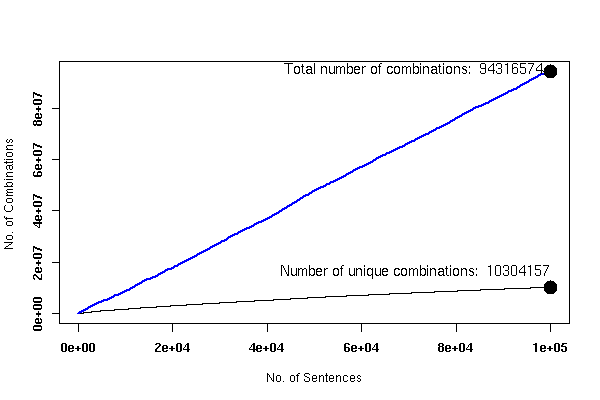
\includegraphics[scale=0.5]{comb.png}	 
	\small The array that stores this information takes exactly $456.797.420$ bytes in $1^{st}$ entry level 
	\end{center}
}
\section{Remaining work}
\frame{
	\frametitle{ Remaining work: Overview }
	\begin{itemize}
	\item The results from \texttt{Colloc} would be much higher quality were the following features implemented in \texttt{Colloc} or in Unitex.
		\begin{itemize}
		\item Detection of boundaries of subordinate clauses
		\item Unification
		\item Disambiguation 
		\item Smarter thresholding
		\item Combining pairs
		\end{itemize}
	\end{itemize}
}
\subsection{Elimination}
\frame{
	\frametitle{ Detection of boundaries of subordinate clauses }
	\begin{itemize}
		\item According to my observations, collocations do not seem to cross subordinate boundaries in a random complex sentence
		\item This problem remains mostly an open problem
		\item However experiences with a restricted corpus with a simpler subordinate boundary detection system deserves attention.
		\item Such a system would drastically reduce the number of bogus combinations, increasing the success rate of the \texttt{Colloc} module and also resulting in remarkable performance gains.
	\end{itemize}
}

\frame{
	\frametitle{ Unification and Disambiguation }
	\begin{itemize}
		\item Pairs like \emph{le table} or pairs that are statistically very significant like \emph{le le}, \emph{le du} are still possible.
		\begin{itemize}
			\item So, applying linguistic operations like unification to eliminate such pairs will improve the \texttt{Colloc} output.
		\end{itemize}
		\item Pairs like \emph{le.DET la.DET} are invalid, (this pair occurs quite frequently in a French corpus) whereas \emph{le.DET la.N} should be kept.
		\begin{itemize}
			\item So, applying disambiguation algorithms to text automata would also improve the \texttt{Colloc} output.
		\end{itemize}
	\end{itemize}
}

\frame{
	\frametitle{ Thresholding }
	\begin{itemize}
		\item An effective elimination method when dealing with frequency data.
		\item An analysis of the first 30.485 sentences of the \texttt{lm94} corpus shows that 85\% of 4.241.598 pairs have frequencies $\leq 3$.
		\item Its weakness is its mercilessness. 
	\end{itemize}
}

\subsection{Combination}
\frame{
	\frametitle{ Combining pairs }
	\begin{itemize}
		\item There exist collocations that span more than two words. 
		\item Current data structure that holds collocation candidates does not contain which pair comes from which sentence.
		\item Once this data structure is expanded, collocations can be combined by studying the correlation of appereance between two pairs
	\end{itemize}
}
\frame{
	\frametitle{ Other Contributions }
	\begin{itemize}

\item Memory management
	\begin{description}
	\item[\texttt{Array}] Judy vs BerkeleyDB
	\item[\texttt{Buffer\_ng}] Read-only file buffer
	\end{description}

\item \texttt{Freq}, a frequency computation module.
	\begin{itemize}
	 \item It takes as input the \texttt{concord.ind} file produced by the \texttt{Locate} module and the \texttt{text.cod} file produced by the tokenizer, it displays the frequency of all the tokens in the vicinity of the given token(s) in the \texttt{concord.ind} file.
	\end{itemize}

\end{itemize}

}

\frame[allowframebreaks]{
	\frametitle{ Bibliography }
	\bibliography{rap.bib}
}

\end{document}
